\chapter{Material suplementario}\label{anx:A}

Este anexo complementa la sección 3.7. Reúne las pruebas de sensibilidad a la elección del umbral de día húmedo: (i) el sesgo histórico de ALADIN respecto de CR2MET en Chile continental con los tres criterios de la Tabla~\ref{tab:criterios} (Tabla~\ref{tab:S1}); (ii) las PDFs históricas por cuenca con cuatro definiciones de umbral (Tabla~\ref{tab:S2}, Figura~\ref{fig:S1}); (iii) el mapa de R₀ local (Figura~\ref{fig:S2}), y (iv) los risk ratios futuros recalculados con 1 mm en ALADIN (Tabla~\ref{tab:S3}, Figura~\ref{fig:S3}). Salvo que se indique lo contrario, se aplican las mismas reglas que en el artículo: período histórico 1980--2014, futuro 2040--2074 (SSP5-8.5), CR2MET interpolado a la grilla de ALADIN, máscara de Chile continental y exclusión de las rachas que tocan el inicio o el fin del período.

\section{Sensibilidad del sesgo histórico a la elección del umbral}\label{sec:S1}

La Tabla~\ref{tab:S1} repite el análisis de mapas de §\ref{sec:pool} con los tres criterios de umbral. Los valores son promedios espaciales sobre las celdas con al menos 30 rachas en ambos productos; la significancia se evalúa con el bootstrap pareado por años de §\ref{sec:pool} (1000 réplicas, IC95).

\begin{longtable}[]{@{}
  >{\raggedright\arraybackslash}p{(\linewidth - 16\tabcolsep) * \real{0.1111}}
  >{\raggedright\arraybackslash}p{(\linewidth - 16\tabcolsep) * \real{0.1111}}
  >{\raggedright\arraybackslash}p{(\linewidth - 16\tabcolsep) * \real{0.1111}}
  >{\raggedright\arraybackslash}p{(\linewidth - 16\tabcolsep) * \real{0.1111}}
  >{\raggedright\arraybackslash}p{(\linewidth - 16\tabcolsep) * \real{0.1111}}
  >{\raggedright\arraybackslash}p{(\linewidth - 16\tabcolsep) * \real{0.1111}}
  >{\raggedright\arraybackslash}p{(\linewidth - 16\tabcolsep) * \real{0.1111}}
  >{\raggedright\arraybackslash}p{(\linewidth - 16\tabcolsep) * \real{0.1111}}
  >{\raggedright\arraybackslash}p{(\linewidth - 16\tabcolsep) * \real{0.1111}}@{}}
\caption[Duración media y t99 de las rachas secas en Chile continental (1980--2014) para CR2MET (1 mm) y ALADIN con cada criterio de umbral]{Duración media y t99 de las rachas secas en Chile continental (1980--2014) para CR2MET (1 mm) y ALADIN con cada criterio de umbral. Δ = ALADIN − CR2MET, calculado píxel a píxel y promediado sobre las celdas comunes. Las dos últimas columnas indican el porcentaje de celdas donde la diferencia es significativa.}\label{tab:S1}\tabularnewline
\toprule\noalign{}
\begin{minipage}[b]{\linewidth}\raggedright
Criterio
\end{minipage} & \begin{minipage}[b]{\linewidth}\raggedright
Métrica
\end{minipage} & \begin{minipage}[b]{\linewidth}\raggedright
CR2MET (días)
\end{minipage} & \begin{minipage}[b]{\linewidth}\raggedright
ALADIN (días)
\end{minipage} & \begin{minipage}[b]{\linewidth}\raggedright
Δ medio (días)
\end{minipage} & \begin{minipage}[b]{\linewidth}\raggedright
Δ mediano (días)
\end{minipage} & \begin{minipage}[b]{\linewidth}\raggedright
\% celdas ALADIN \textless{} CR2MET
\end{minipage} & \begin{minipage}[b]{\linewidth}\raggedright
\% celdas ALADIN \textgreater{} CR2MET
\end{minipage} & \begin{minipage}[b]{\linewidth}\raggedright
Celdas
\end{minipage} \\
\midrule\noalign{}
\endfirsthead
\toprule\noalign{}
\begin{minipage}[b]{\linewidth}\raggedright
Criterio
\end{minipage} & \begin{minipage}[b]{\linewidth}\raggedright
Métrica
\end{minipage} & \begin{minipage}[b]{\linewidth}\raggedright
CR2MET (días)
\end{minipage} & \begin{minipage}[b]{\linewidth}\raggedright
ALADIN (días)
\end{minipage} & \begin{minipage}[b]{\linewidth}\raggedright
Δ medio (días)
\end{minipage} & \begin{minipage}[b]{\linewidth}\raggedright
Δ mediano (días)
\end{minipage} & \begin{minipage}[b]{\linewidth}\raggedright
\% celdas ALADIN \textless{} CR2MET
\end{minipage} & \begin{minipage}[b]{\linewidth}\raggedright
\% celdas ALADIN \textgreater{} CR2MET
\end{minipage} & \begin{minipage}[b]{\linewidth}\raggedright
Celdas
\end{minipage} \\
\midrule\noalign{}
\endhead
\bottomrule\noalign{}
\endlastfoot
i: R₀ global (5,285 mm) & Duración media & 42,1 & 34,0 & −8,2 & −2,2 & 65,3 & 7,5 & 3526 \\
i: R₀ global (5,285 mm) & t99 & 221,1 & 175,3 & −46,3 & −17,2 & 42,6 & 3,5 & 3526 \\
ii: 1 mm en ambos & Duración media & 42,1 & 15,5 & −27,2 & −8,3 & 97,6 & 0,5 & 3549 \\
ii: 1 mm en ambos & t99 & 221,1 & 89,3 & −134,9 & −69,7 & 92,9 & 0,2 & 3549 \\
iii: R₀ local & Duración media & 42,1 & 35,3 & −6,8 & −1,9 & 48,9 & 0,2 & 3471 \\
iii: R₀ local & t99 & 221,1 & 184,0 & −36,0 & −6,5 & 26,0 & 4,4 & 3471 \\
\end{longtable}

Con el mismo umbral de 1 mm (criterio ii), ALADIN acorta las rachas en casi todo el país, porque produce demasiados días con lluvia débil que interrumpen las rachas. Al igualar la frecuencia de días húmedos con un umbral global (criterio i), el sesgo se reduce a menos de un tercio. El umbral local (criterio iii) lo reduce algo más, pero a escala nacional no lo elimina, especialmente en la cola (t99).

\section{PDFs históricas por cuenca con distintos umbrales}\label{sec:S2}

\begin{longtable}[]{@{}
  >{\raggedright\arraybackslash}p{(\linewidth - 14\tabcolsep) * \real{0.1250}}
  >{\raggedright\arraybackslash}p{(\linewidth - 14\tabcolsep) * \real{0.1250}}
  >{\raggedright\arraybackslash}p{(\linewidth - 14\tabcolsep) * \real{0.1250}}
  >{\raggedright\arraybackslash}p{(\linewidth - 14\tabcolsep) * \real{0.1250}}
  >{\raggedright\arraybackslash}p{(\linewidth - 14\tabcolsep) * \real{0.1250}}
  >{\raggedright\arraybackslash}p{(\linewidth - 14\tabcolsep) * \real{0.1250}}
  >{\raggedright\arraybackslash}p{(\linewidth - 14\tabcolsep) * \real{0.1250}}
  >{\raggedright\arraybackslash}p{(\linewidth - 14\tabcolsep) * \real{0.1250}}@{}}
\caption[Estadísticos de duración de las rachas secas por cuenca (1980--2014) para CR2MET con 1 mm y ALADIN con 1 mm (criterio ii), R₀ global (criterio i) y R₀ local (criterio iii)]{Estadísticos de duración de las rachas secas por cuenca (1980--2014) para CR2MET con 1 mm y ALADIN con 1 mm (criterio ii), R₀ global (criterio i) y R₀ local (criterio iii). n = número de rachas.}\label{tab:S2}\tabularnewline
\toprule\noalign{}
\begin{minipage}[b]{\linewidth}\raggedright
Cuenca
\end{minipage} & \begin{minipage}[b]{\linewidth}\raggedright
Serie
\end{minipage} & \begin{minipage}[b]{\linewidth}\raggedright
n
\end{minipage} & \begin{minipage}[b]{\linewidth}\raggedright
Media (días)
\end{minipage} & \begin{minipage}[b]{\linewidth}\raggedright
Mediana (días)
\end{minipage} & \begin{minipage}[b]{\linewidth}\raggedright
p90 (días)
\end{minipage} & \begin{minipage}[b]{\linewidth}\raggedright
p99 (días)
\end{minipage} & \begin{minipage}[b]{\linewidth}\raggedright
Máximo (días)
\end{minipage} \\
\midrule\noalign{}
\endfirsthead
\toprule\noalign{}
\begin{minipage}[b]{\linewidth}\raggedright
Cuenca
\end{minipage} & \begin{minipage}[b]{\linewidth}\raggedright
Serie
\end{minipage} & \begin{minipage}[b]{\linewidth}\raggedright
n
\end{minipage} & \begin{minipage}[b]{\linewidth}\raggedright
Media (días)
\end{minipage} & \begin{minipage}[b]{\linewidth}\raggedright
Mediana (días)
\end{minipage} & \begin{minipage}[b]{\linewidth}\raggedright
p90 (días)
\end{minipage} & \begin{minipage}[b]{\linewidth}\raggedright
p99 (días)
\end{minipage} & \begin{minipage}[b]{\linewidth}\raggedright
Máximo (días)
\end{minipage} \\
\midrule\noalign{}
\endhead
\bottomrule\noalign{}
\endlastfoot
Loa & CR2MET 1 mm & 55 015 & 65,6 & 23 & 185 & 456 & 1419 \\
Loa & ALADIN 1 mm & 129 292 & 27,0 & 12 & 70 & 206 & 1127 \\
Loa & ALADIN R₀ global & 66 267 & 54,6 & 22 & 143 & 360 & 1156 \\
Loa & ALADIN R₀ local & 71 662 & 50,5 & 21 & 127 & 353 & 1150 \\
Maipo & CR2MET 1 mm & 150 209 & 11,0 & 5 & 23 & 119 & 283 \\
Maipo & ALADIN 1 mm & 217 952 & 6,3 & 3 & 14 & 55 & 167 \\
Maipo & ALADIN R₀ global & 181 049 & 8,6 & 4 & 18 & 87 & 194 \\
Maipo & ALADIN R₀ local & 150 900 & 10,6 & 5 & 21 & 124 & 226 \\
Maule & CR2MET 1 mm & 184 462 & 9,5 & 5 & 21 & 83 & 206 \\
Maule & ALADIN 1 mm & 257 231 & 5,8 & 3 & 13 & 39 & 142 \\
Maule & ALADIN R₀ global & 228 077 & 7,3 & 4 & 17 & 57 & 160 \\
Maule & ALADIN R₀ local & 212 397 & 8,2 & 4 & 19 & 67 & 194 \\
Biobío & CR2MET 1 mm & 344 251 & 6,2 & 4 & 14 & 44 & 109 \\
Biobío & ALADIN 1 mm & 423 294 & 4,2 & 3 & 9 & 22 & 79 \\
Biobío & ALADIN R₀ global & 399 130 & 5,3 & 3 & 12 & 34 & 153 \\
Biobío & ALADIN R₀ local & 395 037 & 5,4 & 3 & 12 & 35 & 153 \\
\end{longtable}

\begin{figure}[htbp]
\centering
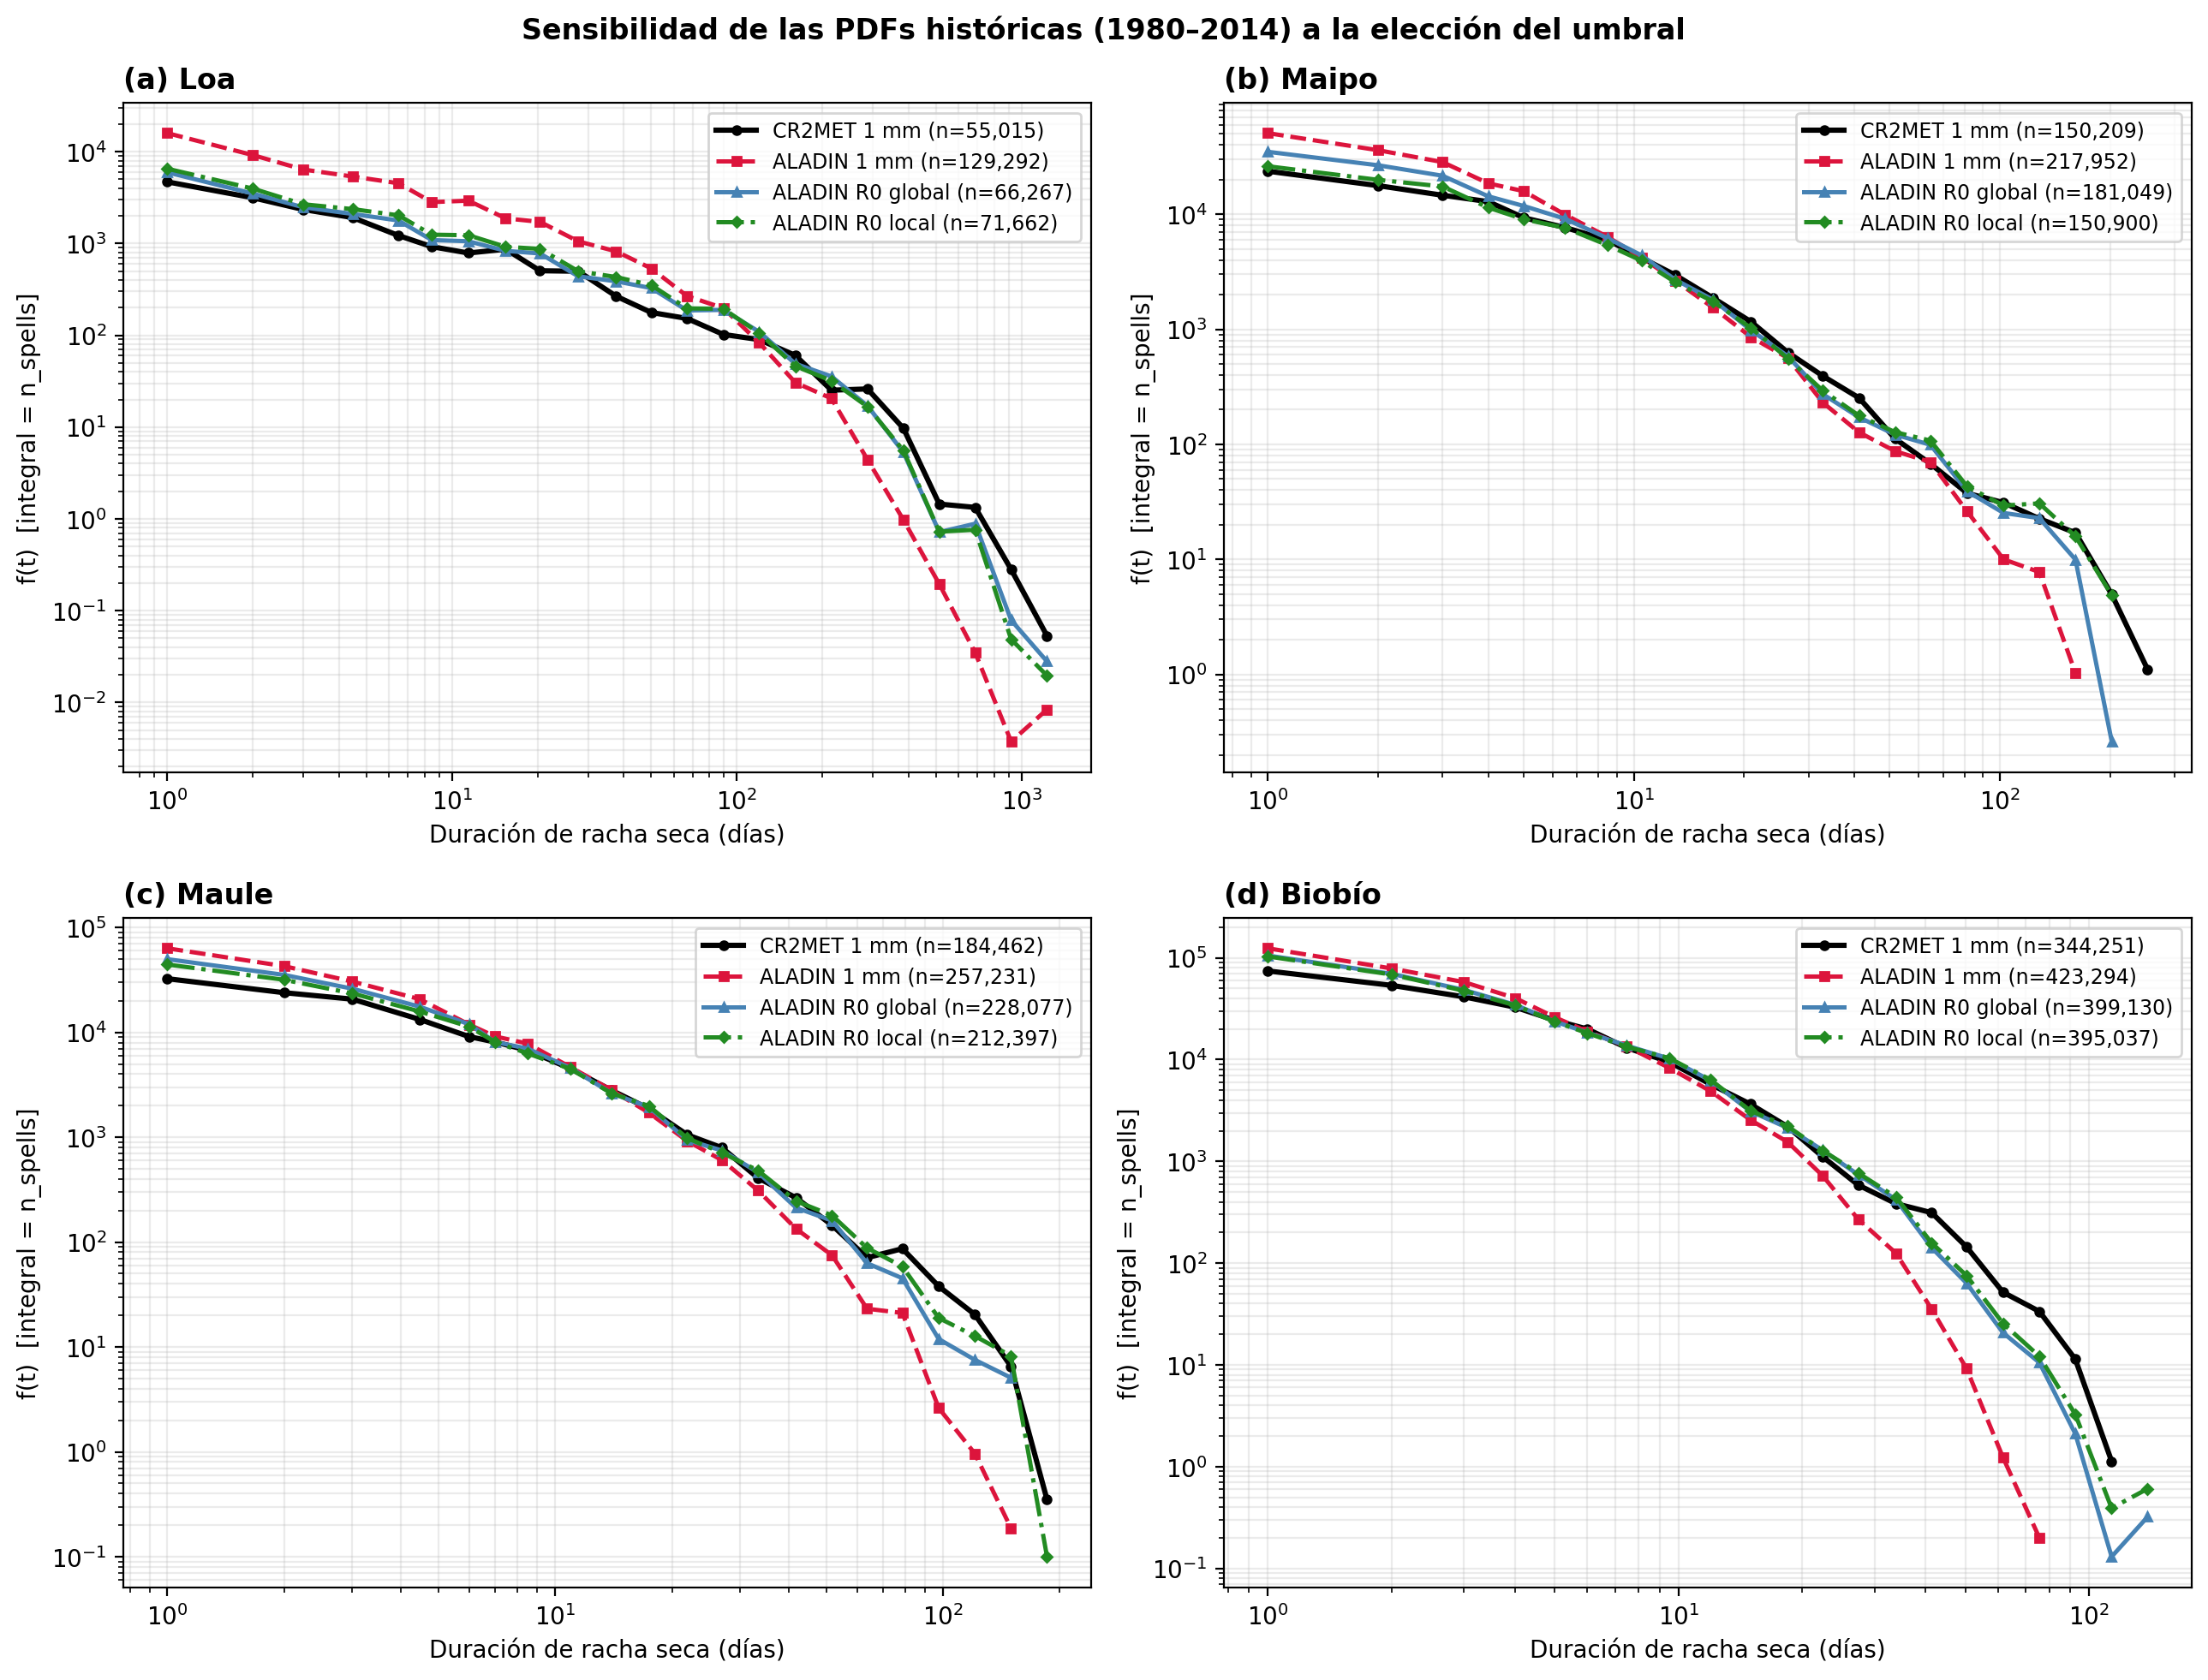
\includegraphics[width=1\linewidth,height=0.72\textheight,keepaspectratio,alt={Sensibilidad de las PDFs históricas (1980--2014) de duración de rachas secas a la elección del umbral de día húmedo, en las cuencas (a) Loa, (b) Maipo, (c) Maule y (d) Biobío. Se comparan CR2MET con 1 mm (negro) y ALADIN con 1 mm (criterio ii, rojo), con R₀ global = 5,285 mm (criterio i, azul) y con R₀ local por píxel (criterio iii, verde). Ejes logarítmicos; los bins son comunes a las cuatro series de cada cuenca (§\ref{sec:pdfs}) y la integral de cada curva es igual a su número de rachas (n).}]{figS1_sensibilidad_umbral_cuencas.png}
\caption[Sensibilidad de las PDFs históricas (1980--2014) de duración de rachas secas a la elección del umbral de día húmedo, en las cuencas (a) Loa, (b) Maipo, (c) Maule y (d) Biobío]{Sensibilidad de las PDFs históricas (1980--2014) de duración de rachas secas a la elección del umbral de día húmedo, en las cuencas (a) Loa, (b) Maipo, (c) Maule y (d) Biobío. Se comparan CR2MET con 1 mm (negro) y ALADIN con 1 mm (criterio ii, rojo), con R₀ global = 5,285 mm (criterio i, azul) y con R₀ local por píxel (criterio iii, verde). Ejes logarítmicos; los bins son comunes a las cuatro series de cada cuenca (§\ref{sec:pdfs}) y la integral de cada curva es igual a su número de rachas (n).}\label{fig:S1}
\end{figure}

Con 1 mm, ALADIN sobreestima las rachas cortas y subestima las largas en las cuatro cuencas. La calibración del umbral acerca las PDFs de ALADIN a la de CR2MET; en Loa, Maule y Biobío la cola de ALADIN sigue terminando antes que la de CR2MET, mientras que en Maipo el R₀ local prácticamente iguala la cola observada (p99 de 124 días frente a 119 días en CR2MET).

\section{Mapa de R₀ local}\label{sec:S3}

\begin{figure}[htbp]
\centering
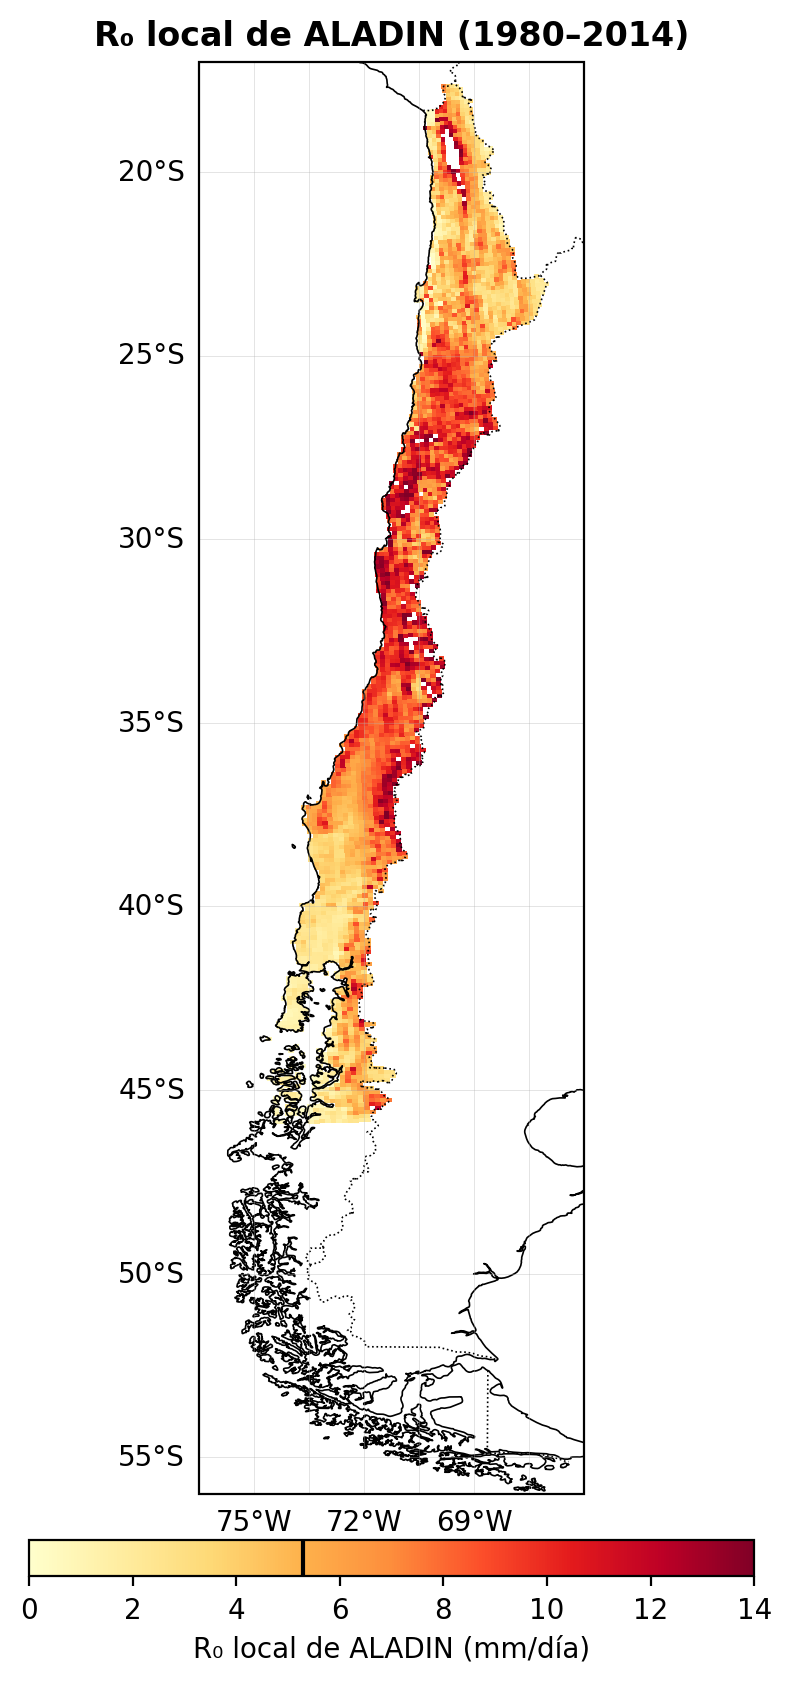
\includegraphics[width=1\linewidth,height=0.72\textheight,keepaspectratio,alt={Umbral local de día húmedo de ALADIN (R₀ local, criterio iii) en 1980--2014. En cada píxel, R₀ local es el umbral para el cual la fracción de días húmedos de ALADIN iguala la de CR2MET con 1 mm, obtenido por bisección. La línea negra en la barra de colores marca el R₀ global (5,285 mm). Los píxeles en blanco (82 de 3587) no tienen solución dentro del intervalo de búsqueda (0--15 mm).}]{figS2_mapa_R0_local.png}
\caption[Umbral local de día húmedo de ALADIN (R₀ local, criterio iii) en 1980--2014]{Umbral local de día húmedo de ALADIN (R₀ local, criterio iii) en 1980--2014. En cada píxel, R₀ local es el umbral para el cual la fracción de días húmedos de ALADIN iguala la de CR2MET con 1 mm, obtenido por bisección. La línea negra en la barra de colores marca el R₀ global (5,285 mm). Los píxeles en blanco (82 de 3587) no tienen solución dentro del intervalo de búsqueda (0--15 mm).}\label{fig:S2}
\end{figure}

El R₀ local tiene una mediana de 6,4 mm (p10 = 2,3 mm; p90 = 11,1 mm) y es inferior al R₀ global en el 39 \% de los píxeles. Los valores más altos se concentran en la zona centro-norte (aproximadamente 28--37 °S) y los más bajos en el extremo norte y en el sur. Esta heterogeneidad es la razón por la que el análisis principal usa un único umbral global (§\ref{sec:definicion}): corrige la frecuencia de días húmedos sin introducir un campo de umbrales que varía de un píxel a otro.

\section{Robustez de la señal futura al umbral}\label{sec:S4}

Para comprobar que el aumento futuro de rachas largas no es consecuencia de la calibración, los risk ratios de §\ref{sec:rr} se recalculan con 1 mm en ALADIN en ambos períodos, manteniendo todas las demás reglas (rachas iniciadas entre marzo y noviembre, bootstrap independiente por años, 1000 réplicas).

\begin{longtable}[]{@{}
  >{\raggedright\arraybackslash}p{(\linewidth - 8\tabcolsep) * \real{0.2000}}
  >{\raggedright\arraybackslash}p{(\linewidth - 8\tabcolsep) * \real{0.2000}}
  >{\raggedright\arraybackslash}p{(\linewidth - 8\tabcolsep) * \real{0.2000}}
  >{\raggedright\arraybackslash}p{(\linewidth - 8\tabcolsep) * \real{0.2000}}
  >{\raggedright\arraybackslash}p{(\linewidth - 8\tabcolsep) * \real{0.2000}}@{}}
\caption[Risk ratio RR(20) = N\_fut(t ≥ 20 d) / N\_hist(t ≥ 20 d) por región con R₀ global (análisis principal, Tabla~\ref{tab:rr}) y con 1 mm en ALADIN]{Risk ratio RR(20) = N\_fut(t ≥ 20 d) / N\_hist(t ≥ 20 d) por región con R₀ global (análisis principal, Tabla~\ref{tab:rr}) y con 1 mm en ALADIN. Entre corchetes, el IC95 bootstrap. En negrita, los aumentos significativos (IC95 completamente sobre 1).}\label{tab:S3}\tabularnewline
\toprule\noalign{}
\begin{minipage}[b]{\linewidth}\raggedright
Región
\end{minipage} & \begin{minipage}[b]{\linewidth}\raggedright
R₀ global: N\_hist → N\_fut
\end{minipage} & \begin{minipage}[b]{\linewidth}\raggedright
R₀ global: RR(20) {[}IC95{]}
\end{minipage} & \begin{minipage}[b]{\linewidth}\raggedright
1 mm: N\_hist → N\_fut
\end{minipage} & \begin{minipage}[b]{\linewidth}\raggedright
1 mm: RR(20) {[}IC95{]}
\end{minipage} \\
\midrule\noalign{}
\endfirsthead
\toprule\noalign{}
\begin{minipage}[b]{\linewidth}\raggedright
Región
\end{minipage} & \begin{minipage}[b]{\linewidth}\raggedright
R₀ global: N\_hist → N\_fut
\end{minipage} & \begin{minipage}[b]{\linewidth}\raggedright
R₀ global: RR(20) {[}IC95{]}
\end{minipage} & \begin{minipage}[b]{\linewidth}\raggedright
1 mm: N\_hist → N\_fut
\end{minipage} & \begin{minipage}[b]{\linewidth}\raggedright
1 mm: RR(20) {[}IC95{]}
\end{minipage} \\
\midrule\noalign{}
\endhead
\bottomrule\noalign{}
\endlastfoot
Coquimbo & 25 367 → 28 458 & \textbf{1,12 {[}1,01; 1,25{]}} & 18 366 → 22 266 & \textbf{1,21 {[}1,06; 1,39{]}} \\
O'Higgins & 7015 → 8096 & 1,15 {[}0,95; 1,40{]} & 4370 → 5132 & 1,17 {[}0,96; 1,47{]} \\
La Araucanía & 2397 → 4118 & \textbf{1,72 {[}1,10; 2,88{]}} & 360 → 1429 & \textbf{3,97 {[}1,46; 16,96{]}} \\
Los Lagos & 601 → 1291 & 2,15 {[}0,90; 8,50{]} & 107 → 27 & 0,25 {[}0,01; 28,07{]} \\
\end{longtable}

\begin{figure}[htbp]
\centering
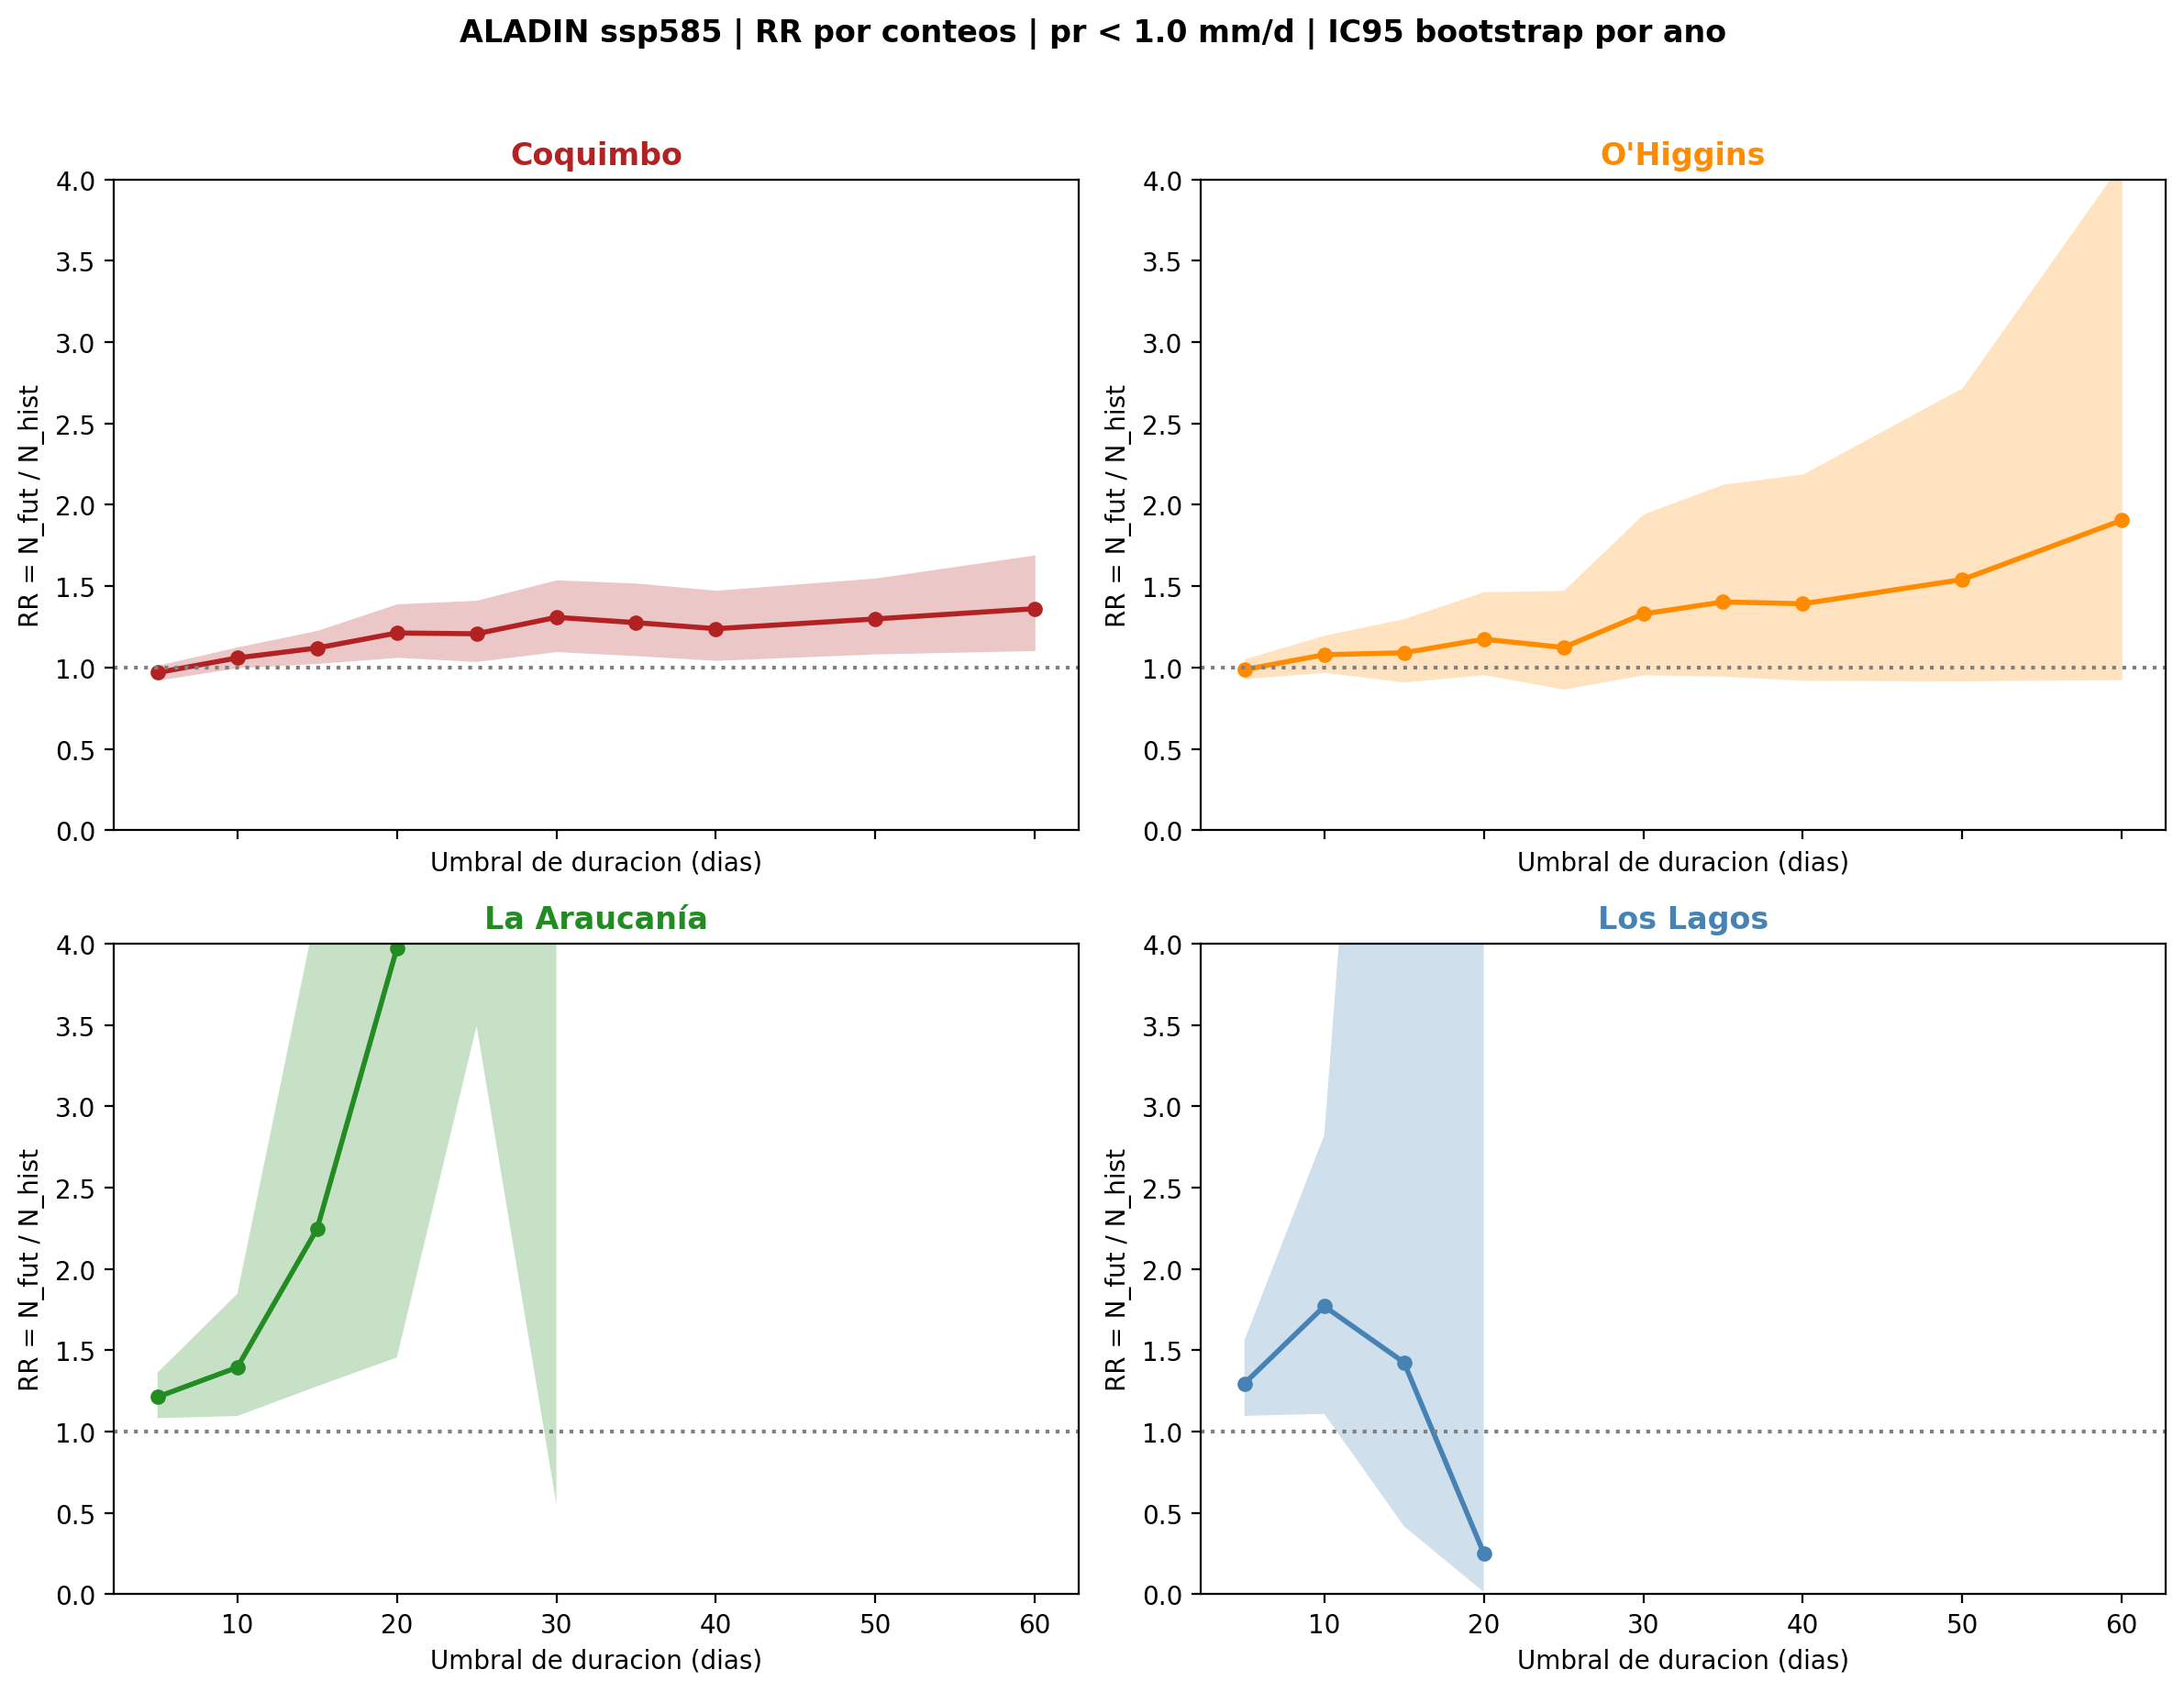
\includegraphics[width=1\linewidth,height=0.72\textheight,keepaspectratio,alt={Risk ratio RR(D) = N\_fut(t ≥ D) / N\_hist(t ≥ D) en función del umbral de duración D para las cuatro regiones, calculado con 1 mm en ALADIN (SSP5-8.5, 2040--2074 frente a 1980--2014). La banda sombreada es el IC95 bootstrap por años; la línea punteada marca RR = 1. Los puntos faltantes corresponden a umbrales sin rachas en el período histórico.}]{figS_rr_curves_aladin_1mm.png}
\caption[Risk ratio RR(D) = N\_fut(t ≥ D) / N\_hist(t ≥ D) en función del umbral de duración D para las cuatro regiones, calculado con 1 mm en ALADIN (SSP5-8.5, 2040--2074 frente a 1980--2014)]{Risk ratio RR(D) = N\_fut(t ≥ D) / N\_hist(t ≥ D) en función del umbral de duración D para las cuatro regiones, calculado con 1 mm en ALADIN (SSP5-8.5, 2040--2074 frente a 1980--2014). La banda sombreada es el IC95 bootstrap por años; la línea punteada marca RR = 1. Los puntos faltantes corresponden a umbrales sin rachas en el período histórico.}\label{fig:S3}
\end{figure}

Con 1 mm, el aumento de rachas largas se mantiene en Coquimbo, donde es significativo para todos los umbrales entre 15 y 60 días, y en La Araucanía. En O'Higgins el RR es mayor que 1 en casi todos los umbrales, pero el intervalo incluye 1, igual que en el análisis principal. En Los Lagos, ALADIN con 1 mm casi no produce rachas de 20 días o más (107 en 35 años), por lo que el RR(20) no es informativo; para duraciones cortas el aumento es significativo (RR(5) = 1,30 {[}1,10; 1,56{]}; RR(10) = 1,77 {[}1,11; 2,82{]}). La señal futura no depende, por lo tanto, de la calibración del umbral en las regiones donde hay rachas suficientes para evaluarla.

\section{Sensibilidad al método de regrillado de CR2MET}\label{sec:S5}

En el análisis principal, CR2MET se interpola linealmente a los centros de celda de ALADIN. Como alternativa, se calculó para cada celda de ALADIN el promedio de las celdas de CR2MET cuyo centro cae dentro de ella (mediana de 6 celdas), y se repitieron la calibración del umbral y los mapas de duración. La precipitación media de Chile en 1980--2014 difiere en 0,24 \% entre ambos métodos (2,597 frente a 2,590 mm día$^{-1}$); por celda, la diferencia se mantiene entre −10 \% y +9 \% en el 90 \% de las celdas, con los mayores valores en zonas de fuerte gradiente orográfico y costero. El promedio por área aumenta la fracción de días húmedos de CR2MET en solo 0,006 puntos porcentuales, por lo que el umbral calibrado prácticamente no cambia. Las diferencias de duración entre ALADIN y CR2MET varían en menos de 0,4 días en la media y menos de 3 días en el percentil 99, en los tres criterios de umbral. Las estadísticas de CR2MET en las cuatro cajas (media, p90 y p99) cambian como mucho 1 día. Las conclusiones no dependen del método de regrillado.

\begin{longtable}[]{@{}lll@{}}
\caption[Comparación entre la interpolación lineal (análisis principal) y el promedio por área de CR2MET sobre la grilla de ALADIN (1980--2014)]{Comparación entre la interpolación lineal (análisis principal) y el promedio por área de CR2MET sobre la grilla de ALADIN (1980--2014). Δ = ALADIN − CR2MET, promedio espacial sobre Chile continental.}\label{tab:S4}\tabularnewline
\toprule\noalign{}
& Interpolación lineal & Promedio por área \\
\midrule\noalign{}
\endfirsthead
\toprule\noalign{}
& Interpolación lineal & Promedio por área \\
\midrule\noalign{}
\endhead
\bottomrule\noalign{}
\endlastfoot
Fracción de días húmedos CR2MET (≥ 1 mm) & 20,945 \% & 20,951 \% \\
R₀ calibrado (mm día$^{-1}$) & 5,285 & 5,280 \\
Δ duración media, criterio i (días) & −8,2 & −7,9 \\
Δ t99, criterio i (días) & −46,3 & −43,7 \\
Δ duración media, criterio ii (días) & −27,2 & −26,9 \\
Δ t99, criterio ii (días) & −134,9 & −132,9 \\
Δ duración media, criterio iii (días) & −6,8 & −6,7 \\
Δ t99, criterio iii (días) & −36,0 & −34,8 \\
\end{longtable}

\section{Sensibilidad de los risk ratios al escenario de emisiones}\label{sec:S6}

Los risk ratios se repitieron con el escenario SSP3-7.0 (2040--2074) de la misma simulación ALADIN, manteniendo el período histórico, el umbral R₀ = 5,285 mm día$^{-1}$ y la restricción a rachas iniciadas entre marzo y noviembre (Tabla~\ref{tab:S5}; Figura~\ref{fig:S4}). En las cuatro regiones, RR(20) es mayor que 1 en ambos escenarios. Con SSP3-7.0 los cambios son algo menores en Coquimbo y La Araucanía, similares en O'Higgins y mayores en Los Lagos. La significancia de valores individuales cambia en los casos cercanos al límite, pero la dirección de la señal es la misma. Como ambos escenarios aún tienen forzamientos similares a mediados de siglo y se dispone de un solo miembro por escenario, las diferencias entre ellos no deben atribuirse al forzamiento.

\begin{longtable}[]{@{}
  >{\raggedright\arraybackslash}p{(\linewidth - 10\tabcolsep) * \real{0.1667}}
  >{\raggedright\arraybackslash}p{(\linewidth - 10\tabcolsep) * \real{0.1667}}
  >{\raggedright\arraybackslash}p{(\linewidth - 10\tabcolsep) * \real{0.1667}}
  >{\raggedright\arraybackslash}p{(\linewidth - 10\tabcolsep) * \real{0.1667}}
  >{\raggedright\arraybackslash}p{(\linewidth - 10\tabcolsep) * \real{0.1667}}
  >{\raggedright\arraybackslash}p{(\linewidth - 10\tabcolsep) * \real{0.1667}}@{}}
\caption{Risk ratio RR(20) = N\_fut(t ≥ 20 d) / N\_hist(t ≥ 20 d) por región con SSP5-8.5 (análisis principal, Tabla~\ref{tab:rr}) y SSP3-7.0. Entre corchetes, el intervalo de confianza del 95 \% por bootstrap por años.}\label{tab:S5}\tabularnewline
\toprule\noalign{}
\begin{minipage}[b]{\linewidth}\raggedright
Región
\end{minipage} & \begin{minipage}[b]{\linewidth}\raggedright
N\_hist
\end{minipage} & \begin{minipage}[b]{\linewidth}\raggedright
SSP5-8.5: N\_fut
\end{minipage} & \begin{minipage}[b]{\linewidth}\raggedright
SSP5-8.5: RR(20)
\end{minipage} & \begin{minipage}[b]{\linewidth}\raggedright
SSP3-7.0: N\_fut
\end{minipage} & \begin{minipage}[b]{\linewidth}\raggedright
SSP3-7.0: RR(20)
\end{minipage} \\
\midrule\noalign{}
\endfirsthead
\toprule\noalign{}
\begin{minipage}[b]{\linewidth}\raggedright
Región
\end{minipage} & \begin{minipage}[b]{\linewidth}\raggedright
N\_hist
\end{minipage} & \begin{minipage}[b]{\linewidth}\raggedright
SSP5-8.5: N\_fut
\end{minipage} & \begin{minipage}[b]{\linewidth}\raggedright
SSP5-8.5: RR(20)
\end{minipage} & \begin{minipage}[b]{\linewidth}\raggedright
SSP3-7.0: N\_fut
\end{minipage} & \begin{minipage}[b]{\linewidth}\raggedright
SSP3-7.0: RR(20)
\end{minipage} \\
\midrule\noalign{}
\endhead
\bottomrule\noalign{}
\endlastfoot
Coquimbo & 25 367 & 28 458 & 1,12 {[}1,01, 1,25{]} & 27 757 & 1,09 {[}0,98, 1,24{]} \\
O'Higgins & 7 015 & 8 096 & 1,15 {[}0,95, 1,40{]} & 8 039 & 1,15 {[}0,97, 1,37{]} \\
La Araucanía & 2 397 & 4 118 & 1,72 {[}1,10, 2,88{]} & 3 679 & 1,53 {[}0,99, 2,47{]} \\
Los Lagos & 601 & 1 291 & 2,15 {[}0,90, 8,50{]} & 1 638 & 2,73 {[}1,13, 11,1{]} \\
\end{longtable}

\begin{figure}[htbp]
\centering
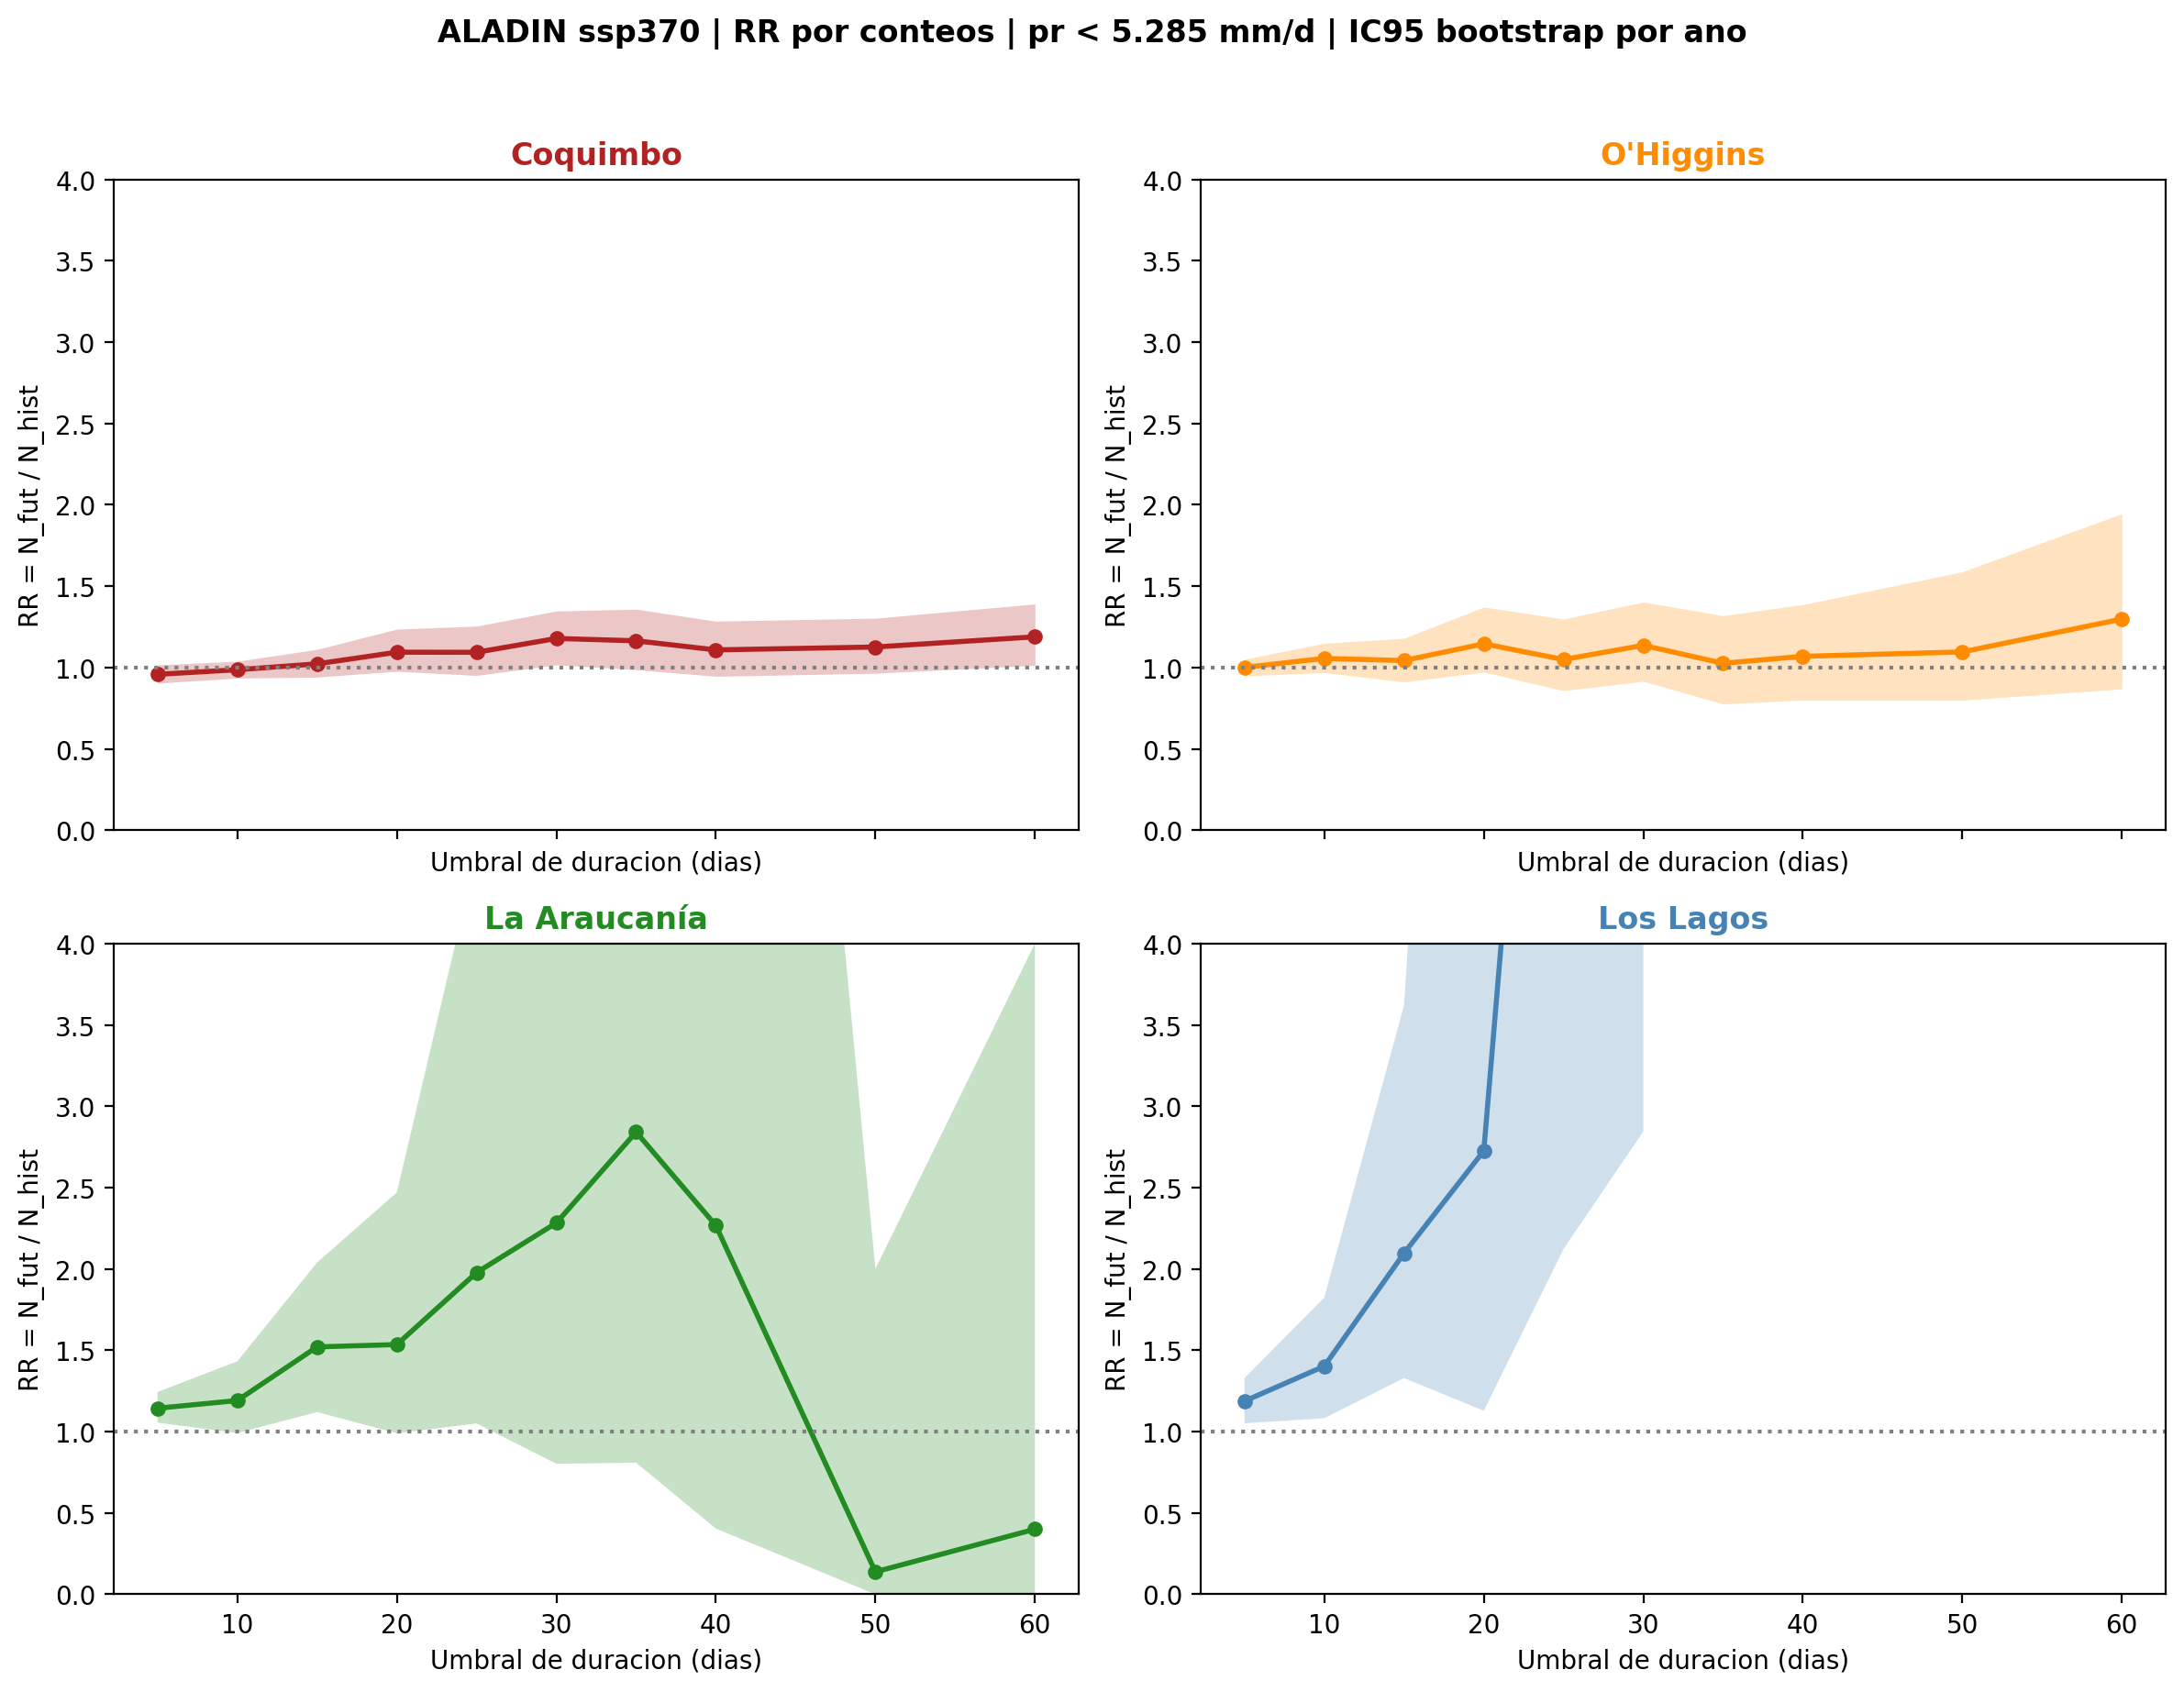
\includegraphics[width=1\linewidth,height=0.72\textheight,keepaspectratio,alt={Risk ratio RR(D) = N\_fut(t ≥ D) / N\_hist(t ≥ D) en función del umbral de duración D para las cuatro regiones, con ALADIN bajo SSP3-7.0 (2040--2074) frente al histórico (1980--2014), R₀ = 5,285 mm día$^{-1}$ y rachas iniciadas entre marzo y noviembre. La banda sombreada es el intervalo de confianza del 95 \% por bootstrap por años.}]{figS_rr_curves_aladin_ssp370.png}
\caption[Risk ratio RR(D) = N\_fut(t ≥ D) / N\_hist(t ≥ D) en función del umbral de duración D para las cuatro regiones, con ALADIN bajo SSP3-7.0 (2040--2074) frente al histórico (1980--2014), R₀ = 5,285 mm día$^{-1}$ y rachas iniciadas entre marzo y noviembre]{Risk ratio RR(D) = N\_fut(t ≥ D) / N\_hist(t ≥ D) en función del umbral de duración D para las cuatro regiones, con ALADIN bajo SSP3-7.0 (2040--2074) frente al histórico (1980--2014), R₀ = 5,285 mm día$^{-1}$ y rachas iniciadas entre marzo y noviembre. La banda sombreada es el intervalo de confianza del 95 \% por bootstrap por años.}\label{fig:S4}
\end{figure}
